The FGSM attack perturbs an image to increase the loss of the classifier on the resulting image. The target label in the original paper \cite{fgsm-original} is always a label with the least probability for an unmodified image. An adversarial example is crafted then by perturbing the unmodified image in a way that the cost function is being maximized.

Let $\pmb \theta$ be the parameters of a model, $\pmb x$ the input to the model, $y$ the target associated with $\pmb x$, and $J (\pmb \theta, \pmb x, y)$ be the cost fucntion used to train the neural network. Then an adversarial perturbation is computed as 
\[ 
\pmb \rho = \epsilon * sign (\nabla_{\pmb x} J(\pmb \theta, \pmb x, y)).
\]

An adversarial example can be crafted then by adding the adversarial perturbation to the original input

\[\pmb x = \pmb x + \pmb \rho .\]
 
The authors evaluate their method on the ImageNet dataset \cite{datasetImageNet}, a dataset used for a large-image recognition task with 1000 classes, and achieve good results for misclassification. Targeted misclassification was not evaluated. Similar results are achieved on the MNIST dataset \cite{datasetMNIST}, a dataset used for a digit-recognition task (0-9), and on the CIFAR-10 dataset \cite{datasetCIFAR10}, a dataset used for a small-image recognition task, also with 10 classes as in MNIST. From Figure \ref{fig:gibbon}, a reader can get the intuition for the attack. For more details, I refer the reader to the original paper.

\begin{figure}[h]
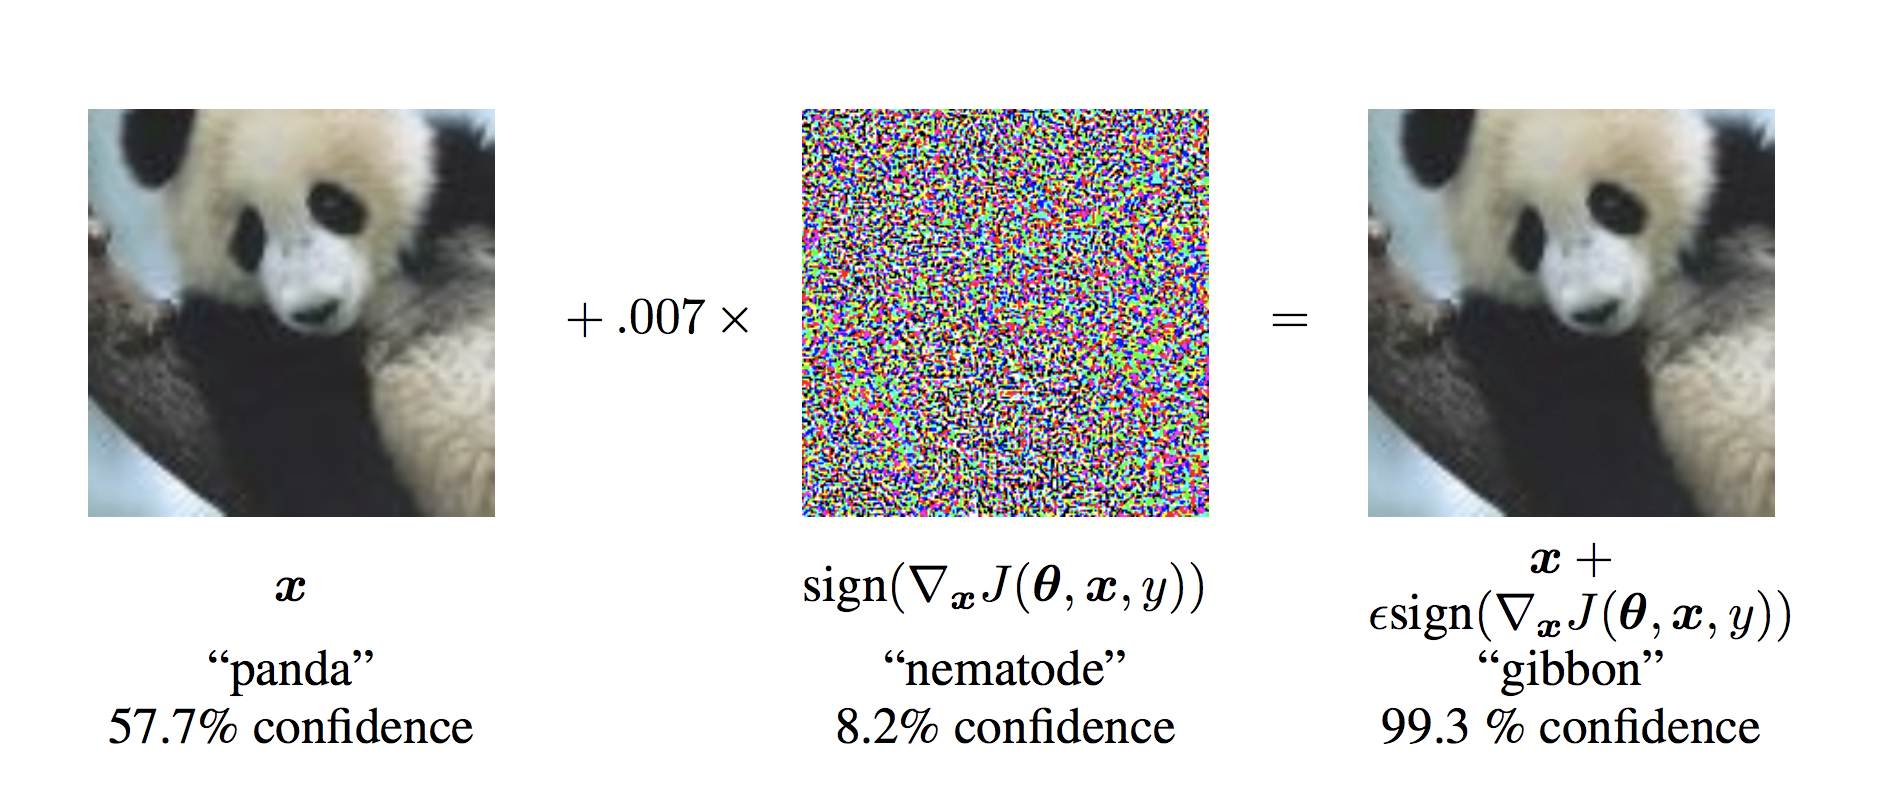
\includegraphics[width=13cm]{gibbon}
\caption{Image taken from the \cite{fgsm-original}}
\label{fig:gibbon}
\end{figure}

